% Opening material before first \section

\subsection*{Speculative apocrypha}



When a group has dominion over an excess supply of resources, its selective pressures will be lessened by ease of replication without struggle, less offspring persisting and passing on variation.

This causes the ever-present potential for variability to become manifest, resulting in a smooth spectrum of divergences and variations. 

As the population expands to meet the supply of resources, the selective pressures begin to return, and what has become a sprawling range of variants once more becomes subject to the formative influence of selection. This begins to ``lock in'' an array of increasingly distinct sub types as the convergence to local optima commences. 

As species begin to move at odds with one-another, there begins competition for the once shared domain. Competitive exclusion may drive types into various distinct sub-niches. But where there is direct overlap, the Matthew effect takes hold, with those species that have some advantage benefiting secondarily from an increase of dominance. 

In this way, what became a huge multiplicity of forms gets reduced. Only a few will persist beyond the day after tomorrow. Only those with some edge, or that were able to secure the early monopoly.

In this way, a substantial easing of selective pressures can cause a stepwise morphological change consistent with the paradim of punctuated equalibria. Much speculation could be made into the possable causes of such a change of conditions. 

The expansion of a genus into a un-exploighted region
Perhaps like the first insects on dry land with a multitude of mosses and small shrubs to feast on. 
Even the first vertebrates that learned how to eat insects. 

Those left after a mass extinction event
Like the small mammals who inherited great swaths of fertile forests after dinosaurs were wiped out at the KT boundary. 

There is speculation that the Cambrian explosion was triggered by some combination of a huge global ice age and a great surplus of oxegen

Speculation has also been made that the evolutionary scale transition from prokaryotes to eukaryotes took place at a time of great surplus oxygen. 

Going beyond the domain of organic life, emergence and divergence of viral models may have followed a similar trajectory. A great variety of models were trialed during a flurry of funding and research into HIV in the early 90s. Over time, only a hand full of these went on to become commonplace.  




Qualitatively, we see that something like this has happened at various times across differing domains. In the first few million years after the cambrian explosion, there were a great variaty of arthropodic forms. 24 classifications have been counted amongst the remains of the Burgess shale. Over time this number was reduced to four main structures: chelicerata (arachnids), crustacea (crustaceans), hexapoda (insects and springtails), and myriapoda (millipedes and centipedes). For about half of the time since then, there were also trilobites, but these eventually dies out. 



\begin{figure}[h!]
    \centering
    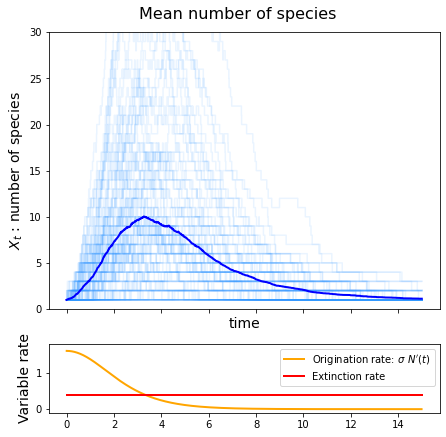
\includegraphics[width=0.7\textwidth]{figures/IMG_ch8/LSMean} % Adjust the width as needed
    \caption{Realisations of the logistic speciation model. Many realisations are shown in light blue. Their average is numerically calculated from these and shown in dark blue. It can clearly be seen that this model exhibits a period of heightened diversification when resources are relatively abundant before seeing a reduction as remaining capacity becomes scarce.  In real evolutionary processes, the latter stage of this procedure might be characterised by a smooth range of types diverging into a few distinct and optimised species which then compete and become subject to the Matthew effect.  Then, either a small number of the fixed types win out, or a number each find slightly different ecological niches to occupy.}
    \label{fig:single_figure}
\end{figure}
